\documentclass[12pt,a4paper]{article}
\usepackage[utf8]{inputenc}
\usepackage[spanish]{babel}
\usepackage{amsmath}
\usepackage{amssymb}
\usepackage{listings}
\usepackage{enumitem}
\usepackage{geometry}
\geometry{margin=2.5cm}
\usepackage[utf8]{inputenc} % allow utf-8 input

\usepackage{listings}
\usepackage{xcolor}

% Define colors
\definecolor{codegreen}{rgb}{0,0.6,0}
\definecolor{codegray}{rgb}{0.5,0.5,0.5}
\definecolor{codepurple}{rgb}{0.58,0,0.82}
\definecolor{backcolour}{rgb}{0.95,0.95,0.92}

% Configure listings
\lstdefinestyle{mystyle}{
  backgroundcolor=\color{backcolour}, 
  commentstyle=\color{codegreen},
  keywordstyle=\color{magenta},
  numberstyle=\tiny\color{codegray},
  stringstyle=\color{codepurple},
  basicstyle=\ttfamily\footnotesize,
  breakatwhitespace=false,   
  breaklines=true,       
  captionpos=b,        
  keepspaces=true,       
  numbers=left,        
  numbersep=5pt,      
  showspaces=false,      
  showstringspaces=false,
  showtabs=false,      
  tabsize=2
}

\lstset{style=mystyle}


\setlength{\parindent}{0pt} % Eliminar sangría de primera línea en todos los párrafos
% add space between paragraphs
\setlength{\parskip}{1em}

% agregar carpeta imagenes
\usepackage{graphicx}
\graphicspath{ {../imagenes/} }


\title{Aprendizaje Reforzado: Guía 3: Programación dinámica}
\author{José Saint Germain}

\begin{document}

\maketitle

\section{Ejercicio 1}

[Programación] Para el proceso de Markov de recompensas (MRP) de la figura,
calcular los valores de los estados  de  forma  iterativa  con  los siguientes 
algoritmos y compare sus convergencias. Considere factor de descuento 
$\gamma <0.9$.

\begin{enumerate}
  \item Actualizar todos los valores a la vez por iteración: $\nu_{k+1} = r + \gamma P \nu_k$, 
  con $\nu_k$, $r$ siendo los  vectores  de  valores  y  recompensas, respectivamente; y $P$ 
  la matriz de probabilidades de transición.
  \item Actualizar el valor de un estado por vez (in place): $\nu_{k+1}(s') = r(s') + \gamma\nu_k(s)$, 
  con $\nu_k(s)$ y $r(s')$ siendo los  valores  y  recompensas correspondientes a los estados 
  $s$ y $s'$, respectivamente.
\end{enumerate}

\subsection{Resolución}

\begin{lstlisting}[language=Python]
R_S2_S1 = 2
R_S1_S2 = 1

P = np.array([
    [0,1], # S1
    [1,0]  # S2
])


def iteracion_sincronica(P, R, gamma, theta=1e-6, max_iterations=1000):
    n_states = P.shape[0]
    V = np.zeros(n_states)
    
    for _ in range(max_iterations):

        V_new = R+gamma * P @ V

        if np.max(np.abs(V_new - V)) < theta:
            break
        V = V_new

    return V

def iteracion_asincronica(P, R, gamma, theta=1e-6, max_iterations=1000):
    n_states = P.shape[0]
    V = np.zeros(n_states)
    
    for i in range(max_iterations):
        delta = 0
        
        for s in range(n_states):
            v = V[s]
            V[s] = R[s] + gamma * np.sum(P[s] * V)
            delta = max(delta, abs(V[s] - v))
        
        if delta < theta:
            break
            
    return V

R = np.array([R_S1_S2, R_S2_S1])  # Recompensas para S1 y S2
gamma = 0.8

V1 = iteracion_sincronica(P, R, gamma)
V2 = iteracion_asincronica(P, R, gamma)
print("Valores de estados (actualizacion simultanea):", V1)
print("Valores de estados (actualizacion in place):", V2)

\end{lstlisting}

\begin{lstlisting}
  Valores de estados (actualizacion simultanea): [7.22221972 7.77777546]
  Valores de estados (actualizacion in place): [7.22222062 7.7777765 ]
\end{lstlisting}

\section{Ejercicio 2} % TODO justificar

En el ejemplo 4.1 (GridWorld, Sutton \& Barto, 2018), donde la política $\pi$ es aleatoria y equiprobable,

\begin{enumerate}
  \item ¿Cuánto vale $ q_\pi(11, \text{down})$?
  \item ¿Cuánto vale $ q_\pi(7, \text{down})$?    
\end{enumerate}

\textbf{Nota:} Utilize $ v(11) = -14$ (fig 4.1 del libro)

Justifique sus respuestas.

\subsection{Resolución}

Sabemos que $q_\pi(s,a) = r + \gamma\nu_\pi(s')$, donde la recompensa siempre es -1
y no es descontada.

$$ q_\pi(s,a) = -1 + \nu_\pi(s') $$

$$ q_\pi(11,\text{down}) = -1 + \nu_\pi(15) = -1 + 0 = -1 $$

$$ q_\pi(7,\text{down}) = -1 + \nu_\pi(11) = -1 - 14 = -15 $$

\section{Ejercicio 3}  % TODO justificar

En el ejemplo 4.1 (GridWorld, Sutton \& Barto, 2018), suponga que se agrega un nuevo estado 15 debajo
del estado 13 y sus acciones: left, up, right y down, lleva al agente a los estados 12,13,14,15, respectivamente.

Considere que las transiciones desde los estados originales no se cambian. ¿Cuánto vale $\nu_\pi(15)$ para la 
política aleatoria y equiprobable? Utilice

\begin{itemize}

\item $\nu(12) = -22$
\item $\nu(13) = -20$
\item $\nu(14) = -14$ (fig 4.1 del libro).
\end{itemize}

Justifique su respuesta.

\subsection{Resolución}

Sabemos que:

$$ \nu_\pi(s) = \sum_a \pi(a|s) [r(s,a) + \gamma \nu_\pi(s')] $$

si la política es aleatoria y equiprobable, y la recompensa siempre es -1:

$$ \nu_\pi(s) = \frac{1}{4} \sum_a [-1 + \nu_\pi(s')] $$

Entonces, $\nu_\pi(15)$ vale:

$$ \nu_\pi(15) = \frac{1}{4} [ -1 + \nu_\pi(12) + -1 + \nu_\pi(13) + -1 + \nu_\pi(14) + -1 + \nu_\pi(15)] $$

tomamos factor común:
$$ \nu_\pi(15) = -1 + \frac{1}{4} [\nu_\pi(12) + \nu_\pi(13) + \nu_\pi(14) + \nu_\pi(15)] $$

remplazamos con los valores conocidos:
$$ \nu_\pi(15) = -1 + \frac{1}{4} [-22 - 20 - 14 + \nu_\pi(15)] $$
$$ \nu_\pi(15) = -1 + \frac{1}{4} [-56 + \nu_\pi(15)] $$
$$ \nu_\pi(15) - \frac{1}{4}\nu_\pi(15) = -1 - 14 $$
$$ \frac{3}{4}\nu_\pi(15) = -15 $$
$$ \nu_\pi(15) = -20 $$

\section{Ejercicio 4}

En el Ejemplo 4.3 (Gambler's problem, Sutton\&Barto, 2018) la política óptima tiene una forma particular 
(ver figura) con máximo en 50. Es decir,  cuando  el  jugador  tiene \$50,  le  conviene apostarlo todo; 
sin embargo, cuando tiene \$51, le conviene apostar \$1. ¿Por qué sucede esto?

\subsection{Resolución}

La moneda no está equilibrada y las probabilidades están en contra del jugador. Por lo tanto,
a medida que la cantidad de lanzamientos aumenta, la probabilidad de ganar disminuye. El jugador 
debe, entonces, jugar con la menor cantidad de lanzamientos posibles: debería
apostar todo su dinero cuando tiene 50, ya que con un lanzamiento puede llegar a 100 y ganar el juego.
Caso contrario, debe apostar lo mínimo para no perder sus posibilidades de ganar.

\section{Ejercicio 5}

[Programación] Implemente el Algoritmo de Iteración de Valores para el Ejemplo 4.3 (Gambler's problem, 
Sutton\&Barto, 2018) para los siguientes casos:

\begin{enumerate}
  \item p(CARA) = 0.25
  \item p(CARA) = 0.55 
\end{enumerate}

Compare los resultados y saque conclusiones.

\subsection{Resolución}

Evaluando la primera situación (p(CARA) = 0.25) en la figura \ref{fig:my_label}, 
vemos que la política óptima no se modifica con respecto al punto anterior (p(CARA) = 0.4).
Esto se debe a que la probabilidad de ganar sigue siendo baja y hay que lograr el objetivo
con la menor cantidad de lanzamientos posibles.

Para el caso de la figura \ref{fig:my_label2} (p(CARA) = 0.55), la política óptima cambia
considerablemente. Ahora, la probabilidad de ganar es mayor y el jugador puede darse el lujo
de apostar el mínimo dinero indispensable (1 dólar) para llegar a 100. De ahí que, sin
importar el capital acumulado, siempre convenga apostar un sólo dólar.

% import figures side by side
\begin{figure}[h!]
  \centering
  \begin{minipage}{0.48\textwidth}
    \centering
    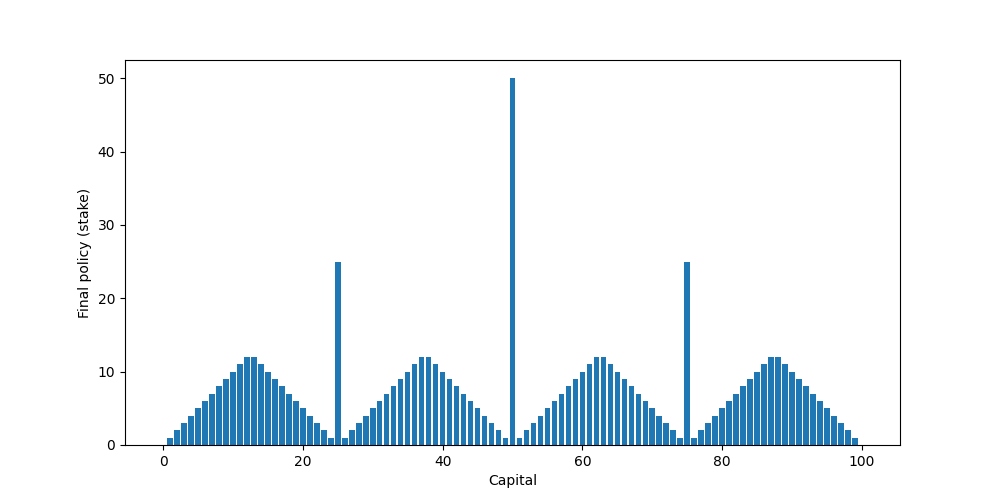
\includegraphics[width=\textwidth]{guia_3_5_p25.png}
    \caption{Política óptima p(CARA) = 0.25}
    \label{fig:my_label}
  \end{minipage}
  \hfill
  \begin{minipage}{0.48\textwidth}
    \centering
    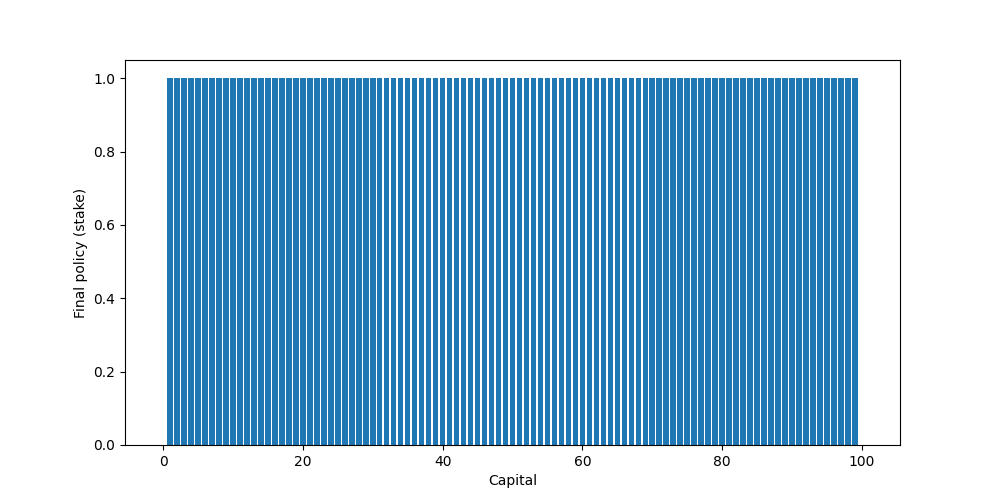
\includegraphics[width=\textwidth]{guia_3_5_p55.png}
    \caption{Política óptima p(CARA) = 0.55}
    \label{fig:my_label2}
  \end{minipage}
\end{figure}

\end{document}